\usetikzlibrary{arrows}
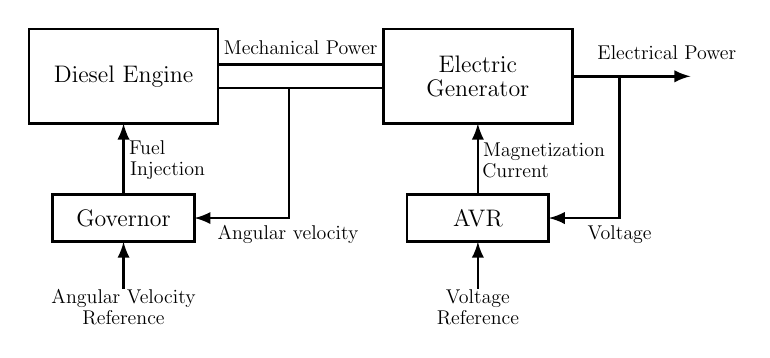
\begin{tikzpicture}[scale=0.6,transform shape]

 \node at (-1.5,1) {\Large{Diesel Engine}};
\draw  [-latex,line width=1pt](-3.5,2) rectangle (0.5,0);
\draw [-latex,line width=1pt] (4,2) rectangle (8,0);
\draw [line width=1pt](0.5,1.25) -- (4,1.25);
\draw [line width=1pt](0.5,0.75) -- (4,0.75);
 \node at (6,1.25) {\Large{Electric}};
 \node at (6,0.75) {\Large{Generator}};
 \node at (-1.5,-2) {\Large{Governor}};
 \node at (6,-2) {\Large{AVR}};
\draw  [-latex,line width=1pt](-3,-1.5) rectangle (0,-2.5);
\draw  [-latex,line width=1pt](4.5,-1.5) rectangle (7.5,-2.5);
\draw [-latex,line width=1pt](-1.5,-1.5) -- (-1.5,0);
\draw [-latex,line width=1pt](2,0.75) -- (2,-2) -- (0,-2);
\draw [-latex,line width=1pt](6,-1.5) -- (6,0);
\draw [-latex,line width=1pt](8,1) -- (10.5,1);
\draw [-latex,line width=1pt](9,1) -- (9,-2) -- (7.5,-2);
\node at (-1,-0.5) {\large{Fuel}};
\node at (-0.57,-1) {\large{Injection}};
\node at (2.25,1.6) {\large{Mechanical Power}};
\node at (1.98,-2.35) {\large{Angular velocity}};
\node at (9,-2.35) {\large{Voltage}};
\node at (10,1.5) {\large{Electrical  Power}};
\node at (7.4,-0.6) {\large{Magnetization}};
\node at (6.8,-1) {\large{Current}};
\draw  [-latex,line width=1pt](-1.5,-3.5) -- (-1.5,-2.5);
\draw  [-latex,line width=1pt](6,-3.5) -- (6,-2.5);
\node at (-1.5,-3.7) {\large{Angular Velocity}};
\node at (-1.5,-4.1) {\large{Reference}};
\node at (6,-3.7) {\large{Voltage}};
\node at (6,-4.1) {\large{Reference}};
\end{tikzpicture}